\documentclass[a4paper]{article}
\usepackage{interspeech2013,amssymb,amsmath,epsfig}
\usepackage{algorithm}
\usepackage{algpseudocode}
\usepackage{array}
\usepackage{url}
\usepackage{enumitem}

% Make it easier to write code inline.
\newcommand\inlinecode[1]{\scriptsize\texttt{#1}\normalsize}

\let\oldurl\url
\makeatletter
\renewcommand*\url{%
        \begingroup
        \let\do\@makeother
        \dospecials
        \catcode`{1
        \catcode`}2
        \catcode`\ 10
        \url@aux
}
\newcommand*\url@aux[1]{%
        \setbox0\hbox{\oldurl{#1}}%
        \ifdim\wd0>\linewidth
                \strut
                \\
                \vbox{%
                        \hsize=\linewidth
                        \kern-\lineskip
                        \raggedright
                        \strut\oldurl{#1}%
                }%
        \else
                \hskip0pt plus\linewidth
                \penalty0
                \box0
        \fi
        \endgroup
}
\makeatother

\setcounter{page}{1}
\sloppy		% better line breaks
\ninept
%SM below a registered trademark definition
\def\reg{{\rm\ooalign{\hfil
     \raise.07ex\hbox{\scriptsize R}\hfil\crcr\mathhexbox20D}}}

%% \newcommand{\reg}{\textsuperscript{\textcircled{\textsc r}}}
\title{ReFr: An Open-Source Reranker Framework}

\let\textquotedbl="

%%%%%%%%%%%%%%%%%%%%%%%%%%%%%% LyX specific LaTeX commands.
\newcommand{\noun}[1]{\textsc{#1}}
%% Because html converters don't know tabularnewline
\providecommand{\tabularnewline}{\\}
\floatstyle{ruled}
\newfloat{algorithm}{tbp}{loa}
\providecommand{\algorithmname}{Algorithm}
\floatname{algorithm}{\protect\algorithmname}

%%%%%%%%%%%%%%%%%%%%%%%%%%%%%% Textclass specific LaTeX commands.
\newenvironment{lyxcode}
{\par\begin{list}{}{
\scriptsize
\setlength{\leftmargin}{0.1in}
\setlength{\rightmargin}{\leftmargin}
\setlength{\listparindent}{0pt}% needed for AMS classes
\raggedright
\setlength{\itemsep}{0pt}
\setlength{\parsep}{0pt}
\normalfont\ttfamily}%
 \item[]}
{\end{list}}

\makeatletter
\def\name#1{\gdef\@name{#1\\}}
\makeatother
\name{{\em Daniel M. Bikel, Keith B. Hall}}

\address{Google Research, New York, NY\\
{\small \tt {\{dbikel,kbhall\}}@google.com}}

%
\begin{document}
\maketitle
%
\begin{abstract}

ReFr is a software architecture for specifying, training and using
reranking models. Reranking models take the n-best output of some
existing system and produce new scores for each of the n hypotheses
that potentially induce a different ranking, ideally yielding better
results than the original system. The Reranker Framework (ReFr for
short) has some special support for building discriminative language
models, but can be applied to any reranking problem.  The framework is
designed with parallelism and scalability in mind, being able to run
on any Hadoop cluster out of the box.  While extremely efficient, ReFr
is also quite flexible, allowing researchers to explore a wide variety
of features and learning methods.


%% ReFr was released in November, 2012 on Google Code
%% (\texttt{http://refr.googlecode.com}), and was originally developed at
%% the 2011 CLSP Summer Workshop, as part of the team working on
%% confusion-based statistical language modeling for machine translation
%% and speech recognition, led by Prof. Brian Roark of OHSU.

%% This paper describes an open-source reranker framework, ReFr, released
%% in November, 2012 on Google Code
%% (\texttt{http://refr.googlecode.com}).  ReFr was originally developed
%% at the 2011 CLSP Summer Workshop, as part of the team working on
%% confusion-based statistical language modeling for machine translation
%% and speech recognition, led by Prof. Brian Roark of OHSU.  Our team
%% was exploring methods that could employ large amounts of unlabeled
%% data, as well as many different types of learning methods and feature
%% types.  Thus, from early on, we wanted our software tools to be built
%% with both parallelism in mind, but also with great flexibility.  ReFr
%% is the result of that effort, implementing a flexible-yet-efficient
%% framework for reranking models, such as for discriminative language
%% modeling, as well as for any reranking or structured prediction
%% problem.
\end{abstract}
\noindent{\bf Index Terms}: language modeling, discriminative language modeling, reranking, structured prediction



%
\section{Introduction}

Creating effective software tools for research is a tricky business.
The classic tension between flexibility and efficiency arises with
greater urgency. We want researchers to be able to try out many
different ideas easily, but we also want them to be able to have a
quick code-test-evaluate cycle.

ReFr grew out of the 2011 Johns Hopkins Summer Workshop, from the team
using automatically generated confusions to synthesize training data
for discriminative language models for speech and machine translation,
led by Prof.\ Brian Roark of OHSU.  That approach required tools that
would scale up to training data sizes orders of magnitude larger than
had previously been used to build discriminative language models, so
we not only needed our training and inference to be inherently fast,
but we needed to design tools with distributed computing in mind from
the outset.

This paper describes the tools we have developed to solve not only the
immediate research problem of exploring confusions for discriminative
language modeling, but also the more general problem of reranking
approaches to speech and language processing, including structured
prediction. We designed ReFr to have the following properites:
\vspace{-0.1in}
\begin{itemize}[noitemsep]
\item ``library quality'' code
\item industrial strength
\item academic flexibility
\item easy exploration of different types of features, different
  update methods (\emph{e.g.}, MIRA-style, direct loss minimization,
  loss-sensitive) and different learning methods (\emph{e.g.},
  perceptron-style, log-linear, kernel methods)
\item modern, object-oriented design, complete with dynamic factories
  and dynamic composition for flexibility
\item parallelizable, especially for distributed-computing
  environments
\end{itemize}
\section{Data Format for I/O}

There are two main choices when building discriminative reranking
models for speech or machine translation: (a) rescore a lattice or
hypergraph or (b) simply use a strict reranking approach applied to
n-best lists. For ReFr, early on we decided to use (b) reranking
n-best lists. The primary reasons were the flexibility this would
allow us in designing features and tools. N-best lists readily allow for
sentence-level features in a way that, say, lattices do not.
Additionally, it is far easier to define generic schemes of passing around
n-best lists than it is for designing schemes to take speech lattices as well
as machine translation hypergraphs or other, problem-specific data types.


\subsection{\label{sub:protobufs}Google Protocol Buffers}

Supervised machine learning is based on the supply of labeled (supervised)
examples from which a model is trained.  A training algorithm is used to induce
the model which best explains the supervised data, while at the same time being
robust to data not seen in the supervised dataset (what is referred to as
the generalization of a model).  The general paradigm is true for all supervised
training algorithms and is also true in the discriminative training algorithms
we use for our experiments in this project. Although not critical when building
a small system which expects relatively little variation in the input data, the
open-source toolkit we have developed is meant to be flexible enough to allow
for a variety of data sources.

In order to avoid the need for overly complex data formats, we have
chosen to adopt a formalism which allows one to augment the input
format, allowing for flexible feature extraction and data manipulation/analysis.
We opted to use a data format which mirrors the data-structures that
are used internally for training. The Google protocol buffers\cite{protobuf}
provide a programming-language independent specification framework
to define data formats. The protocol buffers specification language
is used by the protocol buffer tools to generate source-code for serializing
and deserializing the data stored in the format. Code is generated
to allow for native programming-language encapsulation of the data.
For example, in C++ each item of data is stored in an object based
on a object oriented data specification (a C++ \emph{class}) allowing
for access to the data.\footnote{For the 2011 Johns Hopkins Workshop, we were targeting multiple tasks (ASR and MT), and so our toolkit provides a means to convert from two types of text-based n-best formats, one the output of an ASR system, the other the output of an MT system.  These conversion tools are not only useful in their own right, but serve as example implementations for any developer converting from their own, proprietary format to the Google Protocol Buffer format used by ReFr.}

%% As a by-product of the fact that this workshop targeted multiple tasks
%% (ASR and SMT), we had to address incompatible tools and data formats,
%% which led us to a universal data format. In order to transform
%% data generated in proprietary formats, we developed
%% tools to convert data to our protocol buffer format. These tools are
%% delivered with the open source toolkit in:
%% \begin{verbatim} ./lm-confusion/dataconvert/
%% \end{verbatim} 
%% \begin{description}
%% \item [{FST}] input (Roark's format)
%% \begin{verbatim} ./lm-confusion/dataconvert/asrnbestproto
%% \end{verbatim} 
%% \item [{SMT}] input (K\"{o}hn's format)
%% \begin{verbatim} ./lm-confusion/dataconvert/mtnbestproto
%% \end{verbatim} 
%% \end{description}

%% Each of these tools takes the predefined format as input and outputs a
%% serialized set of protocol buffers.  These are encoded with Base64 encoding and
%% (optionally) compressed (Base64 encoding is needed as protocol-buffers are not
%% self-delimiting).  The disk-based format is able to be manually inspected using
%% the \emph{protoview} tool, found in the repository at:
%%  \begin{verbatim} ./lm-confusion/dataconvert/mtnbestproto \end{verbatim}

\subsection{Protocol Buffer Snippet}

The following is a snippet of the protocol buffer specification for the
training data input format.
\scriptsize
\begin{verbatim}
message CandidateMessage {
  optional CandidateType type = 1;
  optional string rawdata = 2;
  optional FeatureVecMessage feats = 3;
  repeated ScoreMessage score = 4;
}
message CandidateSetMessage {
  // Unique key for this candidate set.
  optional string sourcekey = 1;
  // Index in the original file.
  optional string referencestring = 3;
  repeated CandidateMessage candidate = 4;
  optional int32 goldindex = 5;
  optional int32 bestscoringindex = 6;
}
\end{verbatim}
\normalsize

This specification is automatically compiled into C++, java, or python source code to be
used by the training and inference tools.  The protocol buffer specifications is
delivered with the toolkit (one for the model format and one for the data
format).
\begin{verbatim}
./refr/src/proto/model.proto
./refr/src/proto/data.proto
\end{verbatim}


\section{Core learning framework}

Consider Algorithm \ref{alg:basic-perceptron}, which describes the
training procedure for a generic online-learning algorithm. Each
training example $e_{i}$ comprises a set of \emph{candidate hypotheses},
each of which is projected via some function $\Phi$ into a \emph{feature
space}, $\mathbb{R}^{F}$. We typically think of $\Phi$ as being
a suite of \emph{feature functions}, one per dimension.\emph{ }The\emph{
}model itself is defined as a weight vector in this space, $w$. Decoding,
or inference, is carried out simply by taking the dot product of the
model and a test instance. More generally, any kernel function $\mathcal{K}$
may be used. The training procedure iterates over the training data
$T$---each iteration is called an \emph{epoch}---until the $\Call{NeedToKeepTraining}{}()$
predicate returns \texttt{false}. Often, such a predicate is based
on the average loss of the current model on some held-out development
data $D$, which is the purpose of the $\Call{Evaluate}{D}$ line
in the $\Call{Train}{T}$ procedure.

\begin{algorithm}
Let $e_{i}=\{c_{1},\ldots,c_{k}\}$ be a \emph{training example},
where each $c_{j}$ is a \emph{candidate hypothesis}.

Similarly, let $d_{i}=\left\{ c_{1},\ldots,c_{k}\right\} $ be a held-out
development data example, also consisting of $k$ candidate hypotheses.

Finally, let $\mathcal{K}$ be a \emph{kernel function}.

% redefine \ForAll so it comes out as "foreach"
\renewcommand\algorithmicforall{\textbf{foreach}}
\begin{algorithmic}
\Procedure{Train}{$T = \{e_1, \ldots, e_n\}, D = \{d_1,\ldots,d_m\}$}
  \While{\Call{NeedToKeepTraining}{}()}
    \State \Call{TrainOneEpoch}{$T$}
    \State \Call{Evaluate}{$D$}
  \EndWhile
\EndProcedure
\State
\Procedure{TrainOneEpoch}{$T$}
  \ForAll{training example $e_i$}
    \State \Call{ScoreCandidates}{$e_i$}
    \If {\Call{NeedToUpdate}{}()}
      \State \Call{Update}{}()
    \EndIf
  \EndFor
\EndProcedure
\State
\Procedure{ScoreCandidates}{$e_i$}
  \ForAll{candidate hypothesis $c_j \in e_i$}
    \State $c_j.\texttt{score} \leftarrow K(w_t, c_j)$
  \EndFor
\EndProcedure
\end{algorithmic}

\caption{\label{alg:basic-perceptron}Training algorithm for online-learning
reranking models.}
\end{algorithm}


For the basic perceptron, the model starts out at time step 0 as the
zero vector; that is, $w_{o}=\vec{0}.$ The update is 
\begin{equation}
w_{t+1}=w_{t}+R_{t}\left[\Phi\left(y_{\mathrm{oracle}}\left(e_{i}\right)\right)-\Phi\left(\hat{y}\left(e_{i}\right)\right)\right],\label{eq:perceptron-update}
\end{equation}
 where $y_{\mathrm{oracle}}$ is a function that picks out the hypothesis
towards which we want to bias our model, $\hat{y}$ is a function
that picks out the candidate hypothesis we want to bias our model
against and $R_{t}$ is a \emph{learning rate} or \emph{step size}.
Most often, $y_{\mathrm{oracle}}$ is defined to pick the hypothesis
with the lowest loss relative to some gold-standard truth, and $\hat{y}$
is defined to pick the candidate hypothesis that scores highest under
the current model $w_{t}$. Under this scheme, we would technically
not need a separate $ $$\Call{NeedToUpdate}{}()$ predicate, because
when $y_{\mathrm{oracle}}\left(e_{i}\right)=\hat{y}\left(e_{i}\right)$,
the basic udpate shown in Equation \ref{eq:perceptron-update} is
a ``no op''. In general, however, we would like the flexibility
of defining an arbitrary predicate to determine whether an update
is required.


\subsection{Flexibility without sacrifice}

Most of the variations of this basic learning method involve finding
different ways of defining $R_{t}$, $\Phi$, $y_{\mathrm{oracle}}$
and $\hat{y}$, along with the various procedures and predicates shown
in Algorithm \ref{alg:basic-perceptron}. Therefore, we would like
our Reranker Framework to make it easy for the researcher to define
these various functions, as well as to specify which ones to use at
run-time.

An easy way to design a \emph{flexible} system is to have a basic
interface---let's call it \texttt{Model}---that specifies a \emph{virtual
function} for each operation that a researcher might want to experiment
with. For example, since one might want to experiment with different
definitions for the $\Call{NeedToUpdate}{}()$ method, one could simply
add it to \texttt{Model}. In C++, this would look something like
\begin{lyxcode}
\scriptsize
class~Model~\{

~public:

~~virtual~bool~NeedToKeepTraining()~=~0;

~~virtual~void~TrainOneEpoch(...)~=~0;

~~virtual~bool~NeedToUpdate()~=~0;

~~virtual~void~Update()~=~0;

~~//~...~more~methods~...

\};
\end{lyxcode}
\normalsize
\vspace{-0.2in}

This works well for flexibility, but consider the case where the researcher
wants to experiment with the various, largely orthogonal definitions
of $\Call{NeedToUpdate}{}()$, $\Call{NeedToKeepTraining}{}()$ and
all the other functions. The way one would do this in any object-oriented
setting would be to define a concrete implementation of the \texttt{Model}
interface for each instantiation of the cross product of possible
variants one wanted to explore. Such an approach quickly becomes unwieldy.

A more flexible approach is to use \emph{dynamic composition. }That is, we
keep\emph{ }the idea of a \texttt{Model} interface, but additionally
have each \texttt{Model} instance wrap a set of predicate/manipulator
objects, each of which itself conforms to an interface. Figure \ref{fig:pictorial-view-of-model}
shows a pictorial representation of this scheme. Crucially, a \texttt{Model}
instance \noun{has-a} \texttt{Updater} instance,\texttt{ }and the
\texttt{Updater} interface specifies to use the \texttt{Model} interface,
and similarly for other objects with which a \texttt{Model} is composed.
This mutually recursive relationship is what gives this scheme its
great flexibility without the complexity associated with creating
impossibly many implementations of the \texttt{Model} interface.
%The outline of this approach in C++ is shown in Figure
%\ref{fig:model-with-composition}.
\begin{figure}
\begin{centering}
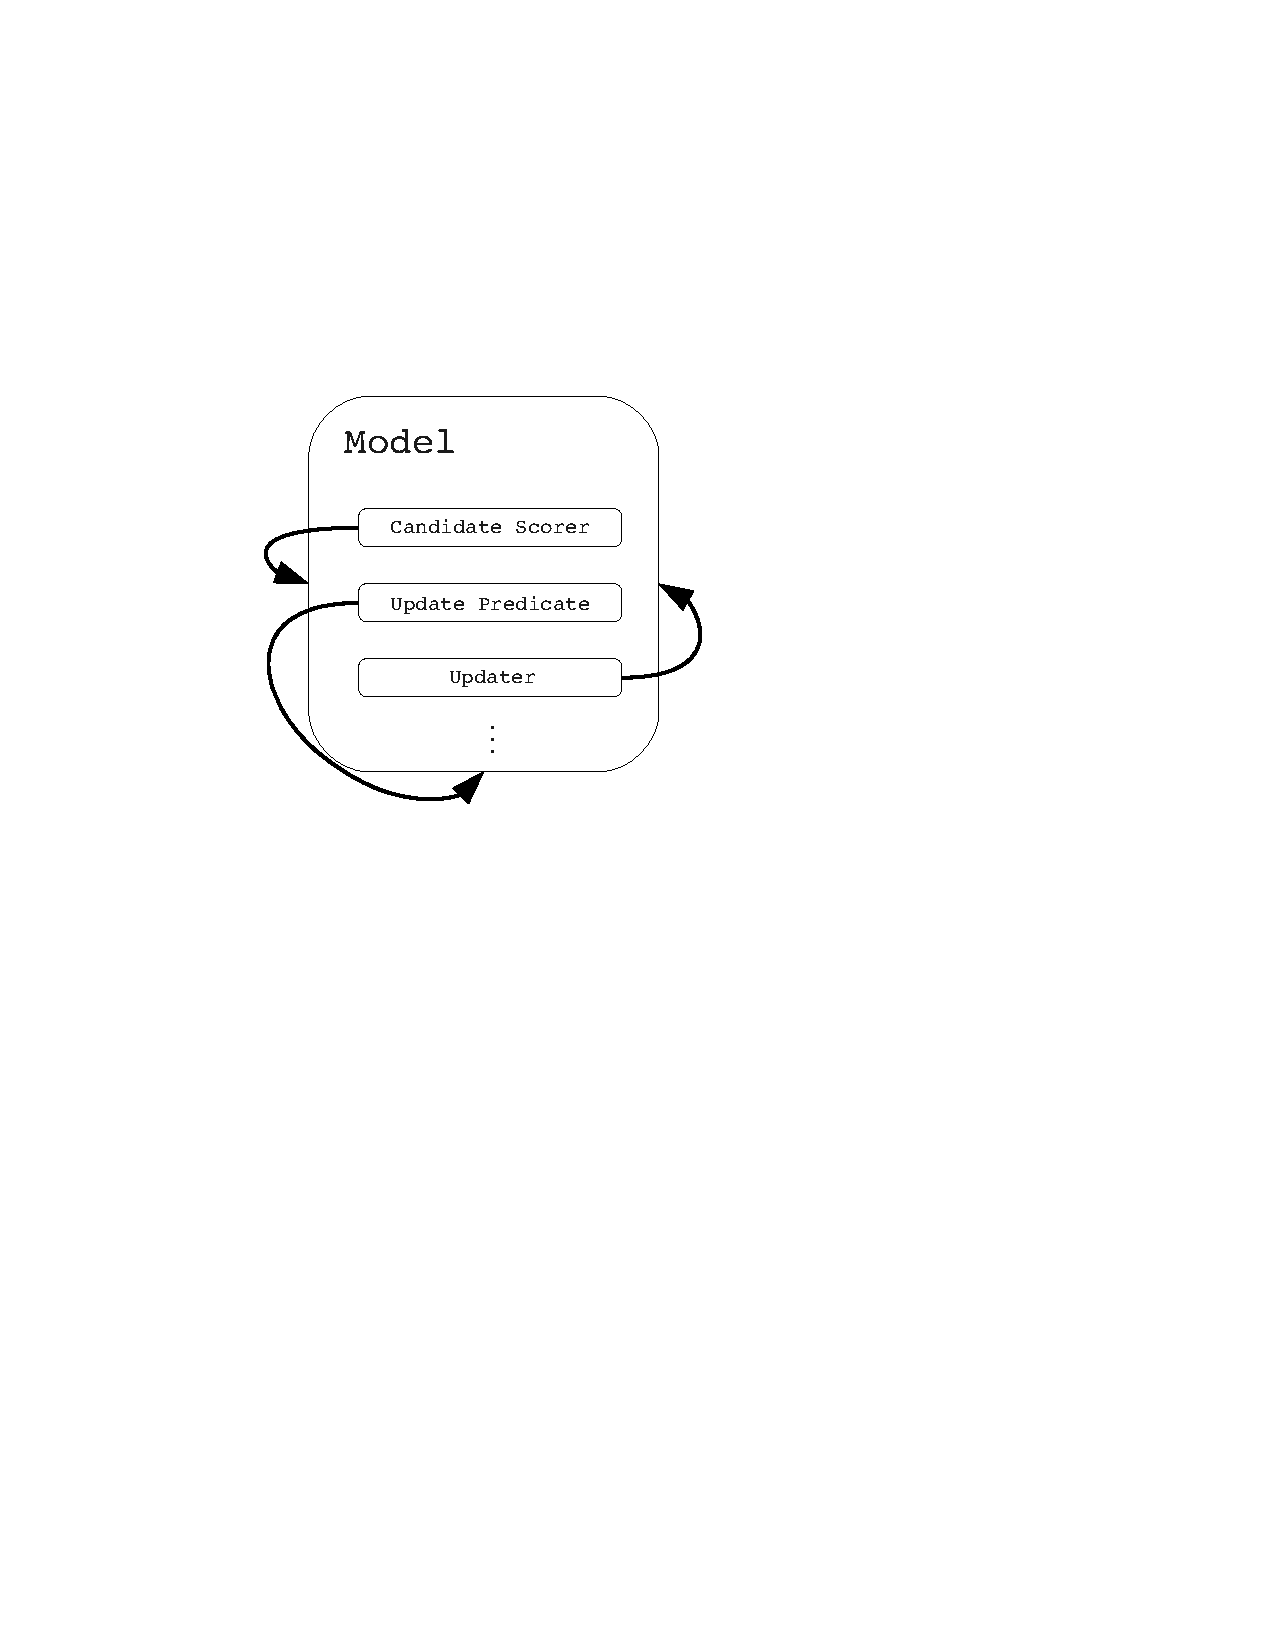
\includegraphics[bb=120bp 400bp 345bp 610bp,clip,scale=0.35]{graphics/model-diagram}
\par\end{centering}

\caption{\label{fig:pictorial-view-of-model}A pictorial view of how a \texttt{Model}
wraps instances of other interfaces that specify the predicates and
functions needed to carry out model training.}
\end{figure}


%% \begin{figure}
%% \begin{lyxcode}
%% class~UpdatePredicate~\{

%% ~public:

%% ~~virtual~bool~NeedToUpdate(const~Model~{*}model)~=~0;

%% \};

%% \

%% class~Updater~\{

%% ~public:

%% ~~virtual~void~Update(Model~{*}model)~=~0;

%% \};

%% \

%% class~CandidateScorer~\{

%% ~public:

%% ~~virtual~void~Score(CandidateSet~\&candidate\_set)~=~0;

%% \};

%% //~...~more~interfaces~to~be~composed~with~Model

%% \

%% class~Model~\{

%% ~public:

%% ~~virtual~bool~NeedToKeepTraining()~=~0;

%% ~~virtual~void~TrainOneEpoch(...)~=~0;

%% ~~virtual~bool~NeedToUpdate()~=~0;

%% ~~virtual~void~Update()~=~0;

%% ~~//~...~more~methods~...

%% ~private:

%% ~~//~data~members

%% ~~Updater~{*}updater\_;

%% ~~UpdatePredicate~{*}update\_predicate\_;

%% ~~CandidateScorer~{*}candidate\_scorer\_;

%% ~~//~...~more~objects~composed~with~Model

%% \};
%% \end{lyxcode}
%% \caption{\label{fig:model-with-composition}The \texttt{Model} interface using
%% dynamic composition with instances of other interfaces.}
%% \end{figure}



\subsection{Dynamic object instantiation}

As we discussed above, we employ dynamic composition to avoid defining
a new subclass of \texttt{Model} every time we wish to explore a new
combination of learning method functions. But how do we actually instantiate
a specific, concrete \texttt{Model} implementation with concrete implementations
of the objects with which it must be composed? We can certainly write
a line---several lines---of code to do this, but if we do that, we
are not much better off than if we had to define a subclass of \texttt{Model}
for every combination we wanted to explore. Moreover, forcing the
user to instantiate objects statically does not even begin to address
the issue of feature function exploration. When we explore different
features---different ways of defining the $F$ feature functions that
constitute $\Phi$---we would ideally like to specify which ones we
wish to employ at run-time.  The basic solution is to use a dynamic factory, but the normal mechanisms of constructing objects by specifying their run-time types via text strings are not powerful or flexible enough for creating complex objects that wrap other objects.

%The basic solution is to use a dynamic factory: a special class with
%a method that takes an object that is easily-specified at run-time,
%such as a \texttt{string}, as a parameter and returns a concrete instance
%of an abstract type, where the concrete type is determined by that
%input parameter. For example, suppose we have our abstract base type
%\texttt{Model} with a concrete implementation called \texttt{PerceptronModel}.
%In C++, we would like to be able to write code like
%\begin{lyxcode}
%//~elsewhere,~perhaps~in~our~main~method
%
%Factory<Model>~model\_factory;
%
%Model~{*}perceptron\_model~=
%
%~~model\_factory.Create(\textquotedbl{}PerceptronModel\textquotedbl{});
%
%//...
%\end{lyxcode}
%Having such \texttt{Factory} instances for dynamic object instantiation
%goes a long way toward making the system easy and flexible, but we
%would ideally like to specify how to construct entire complex objects,
%such as the \texttt{Model} that contains concrete instances of other
%interfaces.


\subsubsection{Dynamic instantiation of complex objects}

Given that C++ is a statically compiled language, we allow the user to specify
the construction of complex objects at run-time via an interpreted language. To
ease the burden on the programmer, this language is very similar to the syntax
used in the initialization phase of C++ constructors. To motivate our choice of
syntax for this interpreted language, let's look at a simple C++ class called
\texttt{Person}, shown in Figure \ref{fig:cpp-person-example}. 
\begin{figure}
\begin{lyxcode}
%//~A~class~to~represent~a~date~in~the~standard\\
%//~Gregorian~calendar.

~class~Date~\{

~~public:

~~~~Date(int~year,~int~month,~int~day)~:

~~~~~~year\_(year),~month\_(month),~day\_(day)~\{~\}

~~private:

~~~~int~year\_;~int~month\_;~int~day\_;

~\};

\

%~//~A~class~to~represent~a~few~facts~about\\
%~//~a~person.

~class~Person~\{

~~public:

~~~~Person(const~string~\&name,~const~Date~\&birthday)~:

~~~~~~name\_(name),~birthday\_(birthday)~\{~\}

~~private:

~~~string~name\_;~Date~birthday\_;

~\};
\end{lyxcode}
\vspace{-0.2in}
\caption{\label{fig:cpp-person-example}A simple C++ example to motivate our
interpreted language syntax.}
\end{figure}


As you can see, the \texttt{Person} class has three data members,
one of which happens to be an instance of another class called \texttt{Date}.
In this case, all of the initialization of a \texttt{Person} happens
in the initialization phase of the constructor\textemdash{}the part
after the colon but before the declaration phase block. By convention,
each parameter to the constructor has a name nearly identical to the
data member that will be initialized from it. If we wanted to construct
a \texttt{Person} instance for someone named \textquotedblleft{}Fred\textquotedblright{}
who was born January 10th, 1990, we could write
the following:
\begin{lyxcode}
Person~fred(\textquotedbl{}Fred\textquotedbl{},~Date(1990,~1,~10))
\end{lyxcode}
If \texttt{Person} were a \texttt{Factory}-constructible type in the
Reranker Framework, we would be able to specify the following as a
specification string to tell the \texttt{Factory} how to construct
a \texttt{Person} instance for Fred:
\begin{lyxcode}
Person(name(\textquotedbl{}Fred\textquotedbl{}),\\
~~~~~~birthday(Date(year(1990),~month(1),~day(10))));
\end{lyxcode}
As you can see, the syntax is very similar to that of C++. It is,
to a first approximation, a combination of the parameter list and
the initialization phase of a C++ constructor.


%% \subsubsection{Interpreted language details}

%% Unfortunately, we cannot get this kind of dynamic instantiation in
%% C++ for free; we need some help from the programmer. However, we have
%% tried to make the burden on the programmer fairly low, using just
%% a handful of macros to help declare a \texttt{Factory} for an abstract
%% base class, as well as to make it easy to make that \texttt{Factory}
%% aware of the concrete subtypes of that base class that it can construct.
%% Finally, each \texttt{Factory}-constructible abstract type needs to
%% implement a single method called \texttt{RegisterInitializers} to
%% specify the names of its data members that this language can initialize.

% Instead of presenting the reader with an inscrutable BNF of the
% grammar, show an example of the interpreter config file.

%% The formal, BNF grammar for our language is shown in Figure \ref{fig:bnf-grammar}.
%% \begin{figure*}
%% \scriptsize
%% \center
%% \begin{tabular}{ll>{\raggedright}p{9cm}}
%% \texttt{<spec>} & \texttt{::=} & \texttt{<type> '(' <member\_init\_list> ')'}\tabularnewline
%% \texttt{<type>} & \texttt{::=} & name of type constructible by this factory\tabularnewline
%% \texttt{<member\_init\_list>} & \texttt{::=} & \texttt{<member\_init> {[} ',' <member\_init> {]}{*} {[}','{]}}\tabularnewline
%% \texttt{<member\_init>} & \texttt{::=} & \texttt{<primitive\_init> | <factory\_init>}\tabularnewline
%% \texttt{<primitive\_init>} & \texttt{::=} & \texttt{<member\_name> '(' <literal> ')'}\tabularnewline
%% \texttt{<member\_name>} & \texttt{::=} & the name of the member to be initialized, as specified by \texttt{<type>}\textquoteright{}s
%% \texttt{RegisterInitializers} method\tabularnewline
%% \texttt{<literal>} & \texttt{::=} & \texttt{<string\_literal> | <double\_literal> | <int\_literal> | <bool\_literal>}\tabularnewline
%% \texttt{<string\_literal>} & \texttt{::=} & a C++ string literal (a string of characters surrounded by double
%% quotes); double quotes and backslashes may be escaped inside a string
%% literal with a backslash; other escape sequences, such as \texttt{\textbackslash{}t}
%% for the tab character, are currently not recognized\tabularnewline
%% \texttt{<double\_literal>} & \texttt{::=} & a string that can be parsed by \texttt{atof}\tabularnewline
%% \texttt{<int\_literal>} & \texttt{::=} & a string that can be parsed by \texttt{atoi}\tabularnewline
%% \texttt{<bool\_literal>} & \texttt{::=} & \texttt{'true' | 'false'}\tabularnewline
%% \texttt{<factory\_init>} & \texttt{::=} & \texttt{<member\_name> '(' <spec> ')'}\tabularnewline
%% \end{tabular}

%% \caption{\label{fig:bnf-grammar}Grammar for interpreted language for dynamic
%% object instantiation in the Reranker Framework.}
%% \end{figure*}



\subsubsection{Putting it all together}

While C++ does not allow dyanamic object instantiation ``for free'',
we have kept the burden on the programmer very low, with macros that
make it easy to declare a \texttt{Factory} for an abstract base class,
as well as macros to make it easy to declare concrete implementations
that should be \texttt{Factory}-constructible.  Also, each
\texttt{Factory}-constructible abstract type needs to implement a
single method called \texttt{RegisterInitializers} to specify the
names of its data members that this language can initialize.


The Reranker Framework contains an extremely portable, lightweight
interpreter of assignment statements in this C++-like language.  The
general form of each assignment statement read by the interpreter is:
\begin{lyxcode}
<variable\_name> = <object>;
\end{lyxcode}
\normalsize
where \inlinecode{<object>} is either a C++ primitive literal---one of
\inlinecode{\{bool,int,double,string\}}---an array of C++ primitives, a
Factory-constructible type or an array of Factory-constructible types
that all have the same abstract type.  Arrays are expressed identically to array literals in C++, by surrounding a comma-separated list of objects with braces.  Underlying, they are implemented using \inlinecode{std::vector}. Figure \ref{fig:interpreter-config} shows an example of a ReFr configuration file.


\begin{figure}
\begin{lyxcode}
\scriptsize
model\_file = \textquotedbl my\_model\_file\textquotedbl;  // model output file

model =\\
~~PerceptronModel(\\
~~~~name(\textquotedbl my model\textquotedbl),\\
~~~~score\_comparator(DirectLossScoreComparator()));

exec\_feature\_extractor =\\
~~ExecutiveFeatureExtractorImpl(\\
~~~~feature\_extractors(\{NgramFeatureExtractor(n(2)),\\
~~~~~~~~~~~~~~~~~~~~~~~~RankFeatureExtractor()\});

training\_efe = exec\_feature\_extractor;\\
dev\_efe = exec\_feature\_extractor;

training\_files = \{\textquotedbl training1.gz\textquotedbl,
\textquotedbl training2.gz\textquotedbl\};\\
devtest\_files = \{\textquotedbl dev1.gz\textquotedbl,
\textquotedbl dev2.gz\textquotedbl\};
\normalsize
\end{lyxcode}
\vspace{-0.2in}
\caption{\label{fig:interpreter-config}An example ReFr configuration file, read by its \inlinecode{Interpreter} class.}
\end{figure}

% This section needs to be MUCH shorter.

%% The Reranker Framework defines a common base class for all feature
%% extractors called \texttt{FeatureExtractor}. Now, \texttt{FeatureExtractor}
%% instances are \texttt{Factory}-constructible, and so the \texttt{FeatureExtractor}
%% class ensures its concrete subclasses have a \texttt{RegisterInitializers}
%% method. One of the concrete implementations of \texttt{FeatureExtractor}
%% provided with the Reranker Framework is \texttt{NgramFeatureExtractor},
%% which extracts n-gram features from a training or test instance's
%% text on the fly.%
%% \footnote{This is one of the pieces of the Reranker Framework that is specialized
%% for discriminative language modeling.%
%% } That class has two data members that can be initialized by a factory,
%% one required and one optional. To show you how easy it is to \textquotedblleft{}declare\textquotedblright{}
%% data members that need initialization, here is the exact code from
%% the \texttt{NgramFeatureExtractor::RegisterInitializers} method:
%% \begin{lyxcode}
%% \tiny
%% virtual~void~RegisterInitializers(Initializers~\&initializers)~\{

%% ~~bool~required~=~true;

%% ~~initializers.Add(\textquotedbl{}n\textquotedbl{},~\&n\_,~required);

%% ~~initializers.Add(\textquotedbl{}prefix\textquotedbl{},~\&prefix\_);

%% \}
%% \normalsize
%% \end{lyxcode}
%% The above code says that the \texttt{NgramFeatureExtractor} has a
%% data member \texttt{n\_}, which happens to be an \texttt{int}, that
%% is required to be initialized when an \texttt{NgramFeatureExtractor}
%% instance is constructed by a \texttt{Factory}, and that the name of
%% this variable will be \texttt{\textquotedbl{}n\textquotedbl{}} as
%% far as the factory is concerned. It also says that it has a data member
%% \texttt{prefix\_}, which happens to be of type \texttt{string}, whose
%% factory name will be \texttt{\textquotedbl{}prefix\textquotedbl{}},
%% and that is not required to be present in a specification string for
%% an \texttt{NgramFeatureExtractor}.

%% Given the grammar described earlier, the following are all legal specification
%% strings for constructing \texttt{NgramFeatureExtractor} instances:
%% \begin{lyxcode}
%% NgramFeatureExtractor(n(3))

%% NgramFeatureExtractor(n(2),~prefix(\textquotedbl{}foo:\textquotedbl{}))

%% NgramFeatureExtractor(prefix(\textquotedbl{}bar\textquotedbl{}),~n(4))

%% NgramFeatureExtractor(n(2),)
%% \end{lyxcode}
%% As you can see, the order of member initializers is not important
%% (because each has a unique name), and you can optionally put a comma
%% after the last initializer. The following are illegal specification
%% strings for \texttt{NgramFeatureExtractor} instances:
%% \begin{lyxcode}
%% //~Illegal~specification~strings:

%% NgramFeatureExtractor(prefix(\textquotedbl{}foo\textquotedbl{}))

%% NgramFeatureExtractor()

%% NgramFeatureExtractor(n(3),~prefix(4))
%% \end{lyxcode}
%% In the first two cases, the specification strings are missing the
%% required variable n, and in the final case, the optional prefix member
%% is being initialized, but with an int literal instead of a string
%% literal.

%% As a more complex example, let us consider the abstract base class
%% \texttt{Model}, which is also \texttt{Factory}-constructible. Each
%% \texttt{Model} uses an instance of a comparator interface to determine
%% the \textquotedblleft{}gold\textquotedblright{} and top-scoring candidates
%% when training. This is the primary means by which the Reranker Framework
%% allows the user to specify a way of picking $\hat{y}$ in Equation
%% \ref{eq:perceptron-update}. The specification strings for constructing
%% \texttt{Model} instances reveal how recursion is used for constructing
%% complex objects in this interpreted language. For example, to construct
%% a \texttt{PerceptronModel} instance with a \texttt{DirectLossScoreComparator}
%% , one would use the following specification string:
%% \begin{lyxcode}
%% PerceptronModel(\\
%% ~~name(\textquotedbl{}MyPerceptronModel\textquotedbl{}),\\
%% ~~score\_comparator(DirectLossScoreComparator()))
%% \end{lyxcode}
%% The first member initialization, for the member called \texttt{name},
%% specifies the unique name you can give to each \texttt{Model} instance
%% (which is strictly for human consumption). The second member initialization,
%% for the member called \texttt{score\_comparator}, overrides the default
%% comparator used to compare candidate hypothesis scores. This second
%% member is also an example of one \texttt{Factory}-constructible object
%% being constructed as a data member of another \texttt{Factory}-constructible
%% object.


\subsection{Feature extraction}

Another area that should be maximally flexible and yet easy to use
is the specification of features, that is, the $\Phi$ of Equation
\ref{eq:perceptron-update}. If one already has features encoded in
either Roark's or K\"{o}hn's format, one may use the tools described in
\S\ref{sub:protobufs}. That is one of the ways in which one can
incorporate pre-computed features. Often, it is preferable to define
many feature functions and choose among them on the fly. The Reranker
Framework makes this easy, once again using the interpreted language
for specifying which feature extractors to use, as demonstrated by
the \texttt{NgramFeatureExtractor} example of the previous section.
For even more flexibility, one might want to combine features that
are extracted on the fly with different sets of features that have
been precomputed but are sitting in separate files on disk. This scenario,
too, is made easy by the Reranker Framework, which provides specialized
\texttt{FeatureExtractor} implementations that can ``extract'' precomputed
features from files.%
\footnote{The class \texttt{AbstractFileBackedFeatureExtractor} is the base
class for such feature extractors.%
} The class \texttt{ExecutiveFeatureExtractor} handles the run-time
construction and initialization of a suite of \texttt{FeatureExtractor}\emph{
}instances to be run on each problem instance at run-time.
%It uses an internal \texttt{Factory} instance to accomplish this. 


\subsection{Training}

The traditional way to train a model for classification, reranking
or structured prediction is to read the training data into memory
and then iterate over it until training is complete. This way of training
tends to minimize the time spent doing I/O and maximize the efficiency
of training, but at the expense of memory. As Algorithm \ref{alg:basic-perceptron}
shows, the basic perceptron algorithm involves ``online'' updating,
and thus it is possible to read in each training example from file
each time it is needed, only keeping the model's parameters persistently
in memory. The Reranker Framework allows both the memory-intensive
way of training as well as this ``streaming mode'' version of training.
Crucially, training in ``streaming mode'' is essential to providing
the distributed training framework, described in the next section.


\section{Cluster-based distributed training}

Learning techniques which are able to exploit unlabeled examples for
training models often fall under the name semi-supervised learning;
however, there are additional techniques which make use of unlabeled
data (e.g., distance supervision\cite{mintz09}). Inducing training
data from unlabeled text for discriminative modeling is another technique which
can result in a relatively large set of training data (depending on the
technique, this set is unbounded). Addressing the issue of huge sets of training
data, we have developed a distributed training paradigm which can be executed on
a cluster of compute nodes via the Hadoop MapReduce training framework.

The most direct approach to distributed, supervised learning is to
split the training data into smaller subsets and process each of these
subsets on a separate computing node (either multiple nodes on a single
machine or across multiple machines in a cluster computing environment).
The differences between distributed learning (and distributed optimization)
algorithms arise at this point; the primary questions being,
 \textquotedbl{}what computation is performed on each subset and how does this
contribute to a global model.  \textquotedbl{}
One of the solutions is to distribute the data, train multiple
independent models and then average their parameters; a technique known
as parameter mixtures \cite{gmann2009}. Another technique is to use a batch training
technique which collects statistics from each of the subsets, make
an update to a global model and sends that model back to the clusters
for the next iteration (epoch) of training. This is applied in the
standard distributed gradient computation techniques.

The structured perceptron \cite{Collins02b} and it's variants have proven to
be effective in supervised, discriminative language modeling work
\cite{Roark07}.  We have centered the development of 
our open-source discriminative learning toolkit around perceptron-style
algorithms, which are, by definition, online learning algorithms. Identifying the
optimal solution for a distributed online optimization algorithm is still an open
research question. We borrow from our previous work on distributed perceptron
training in \cite{mcdonald10distributed,hall10distributed} and use the
\emph{Iterative Parameter Mixtures} algorithm for distributed computation.

\subsection{Iterative Parameter Mixtures}
\begin{algorithm}[h]
\scriptsize
\caption{Iterative Parameter Mixtures Perceptron}
\label{alg:IPM}
\begin{algorithmic}
  \State \Comment{Break $S$ into $K$ partitions}
  \State $S=\{D^{1},\ldots,D^{j},\ldots,D^{K}\}$ \Comment{e.g., $D^{1}={(x_{1}^{1},y_{1}^{1})\ldots(x_{S/K}^{1},y_{S/K}^{1})}$}
  \State $t=0$
  \Repeat
    \State $t=t+1$
    \For {$j=1\ldots K$} \Comment{Process in parallel}
      \State $\theta_{t}^{j}=\theta_{t-1}$
      \For{$i=1\ldots|D^{j}|$}
        \If {$\hat{y}_{i}\ne y_{i}$}
          \State \Comment{Update model Parameters}
          \State $\theta_{t}^{j}=\theta_{t}^{j}+\Phi(y_{i})-\Phi(\hat{y}_{i})$
        \EndIf
      \EndFor
      \State $\Delta^{j}=\theta_{t}^{j}-\theta_{t-1}$
    \EndFor
    \For{$l=1\ldots|w|$} \Comment{For each feature in the model (can be done in parallel)}
      \State $\theta_{t}(l)=\theta_{t-1}(l)+\frac{1}{K}\sum_{j}\Delta^{j}(l)$
    \EndFor
  \Until{converged}
   \end{algorithmic} 
\normalsize
\end{algorithm}

The iterative parameter mixtures (IPM) perceptron trainer is a distributed
approximation to the standard perceptron algorithm. The general idea
is to perform many partial optimizations over subsets of the training
data followed by a synchronization of the updated models form each of
the partial optimizations.  This process repeats during each epoch of training.

Algorithm~\ref{alg:IPM} shows the IPM perceptron algorithms as presented
in \cite{mcdonald10distributed}. We split the data into $K$
partitions: $D^{1}$ through $D^{K}$. Each of these
partitions is processed independently on separate machines. During each iteration
of training, each of these machines makes one pass through its partition
of data, performing the standard structured perceptron up-date to its internal
model.  After all partitions have been processed, each machine sends its
version of the global model to another set of machines responsible for averaging
the models.  In order to do this later
merging step, we partition each of the models based on their feature ids (e.g.,
each of these \emph{merging} machines merges a subset of the feature space).
Each machine will start its next epoch of training with the globally merged
model.

There are some subtleties in the IPM algorithm which we have left out
in this presentation (e.g., details of the parameter averaging).
The implementation we are providing with the open source toolkit uses
an error-weighted average (the contribution of each partitions
average is weighted by the number of errors made over that partition in the most
recent training epoch).  This has the added benefit of being no slower to
converge (in number of epochs over the training data) than that standard
perceptron algorithm.

\subsection{Hadoop Implementation}
\begin{figure}[th]
\centering 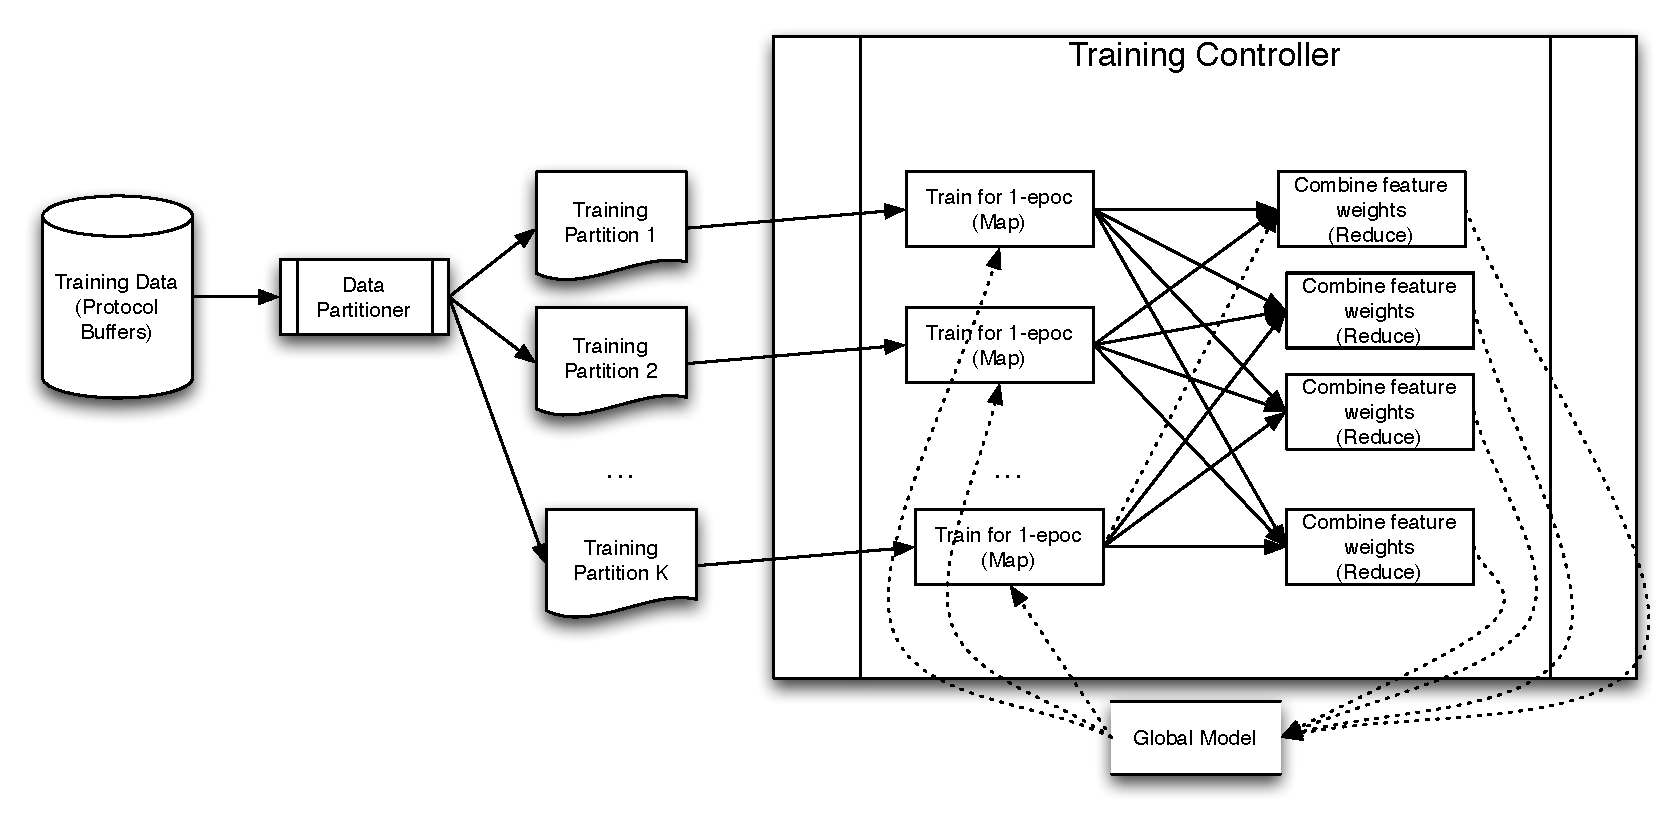
\includegraphics[width=.5\textwidth]{graphics/mapreduceflow} 
\caption{\label{fig:hadoopipm}Flow of Iterative Parameter Mixtures algorithm implemented in {ReFr}.}
\end{figure}

The iterative parameter mixtures algorithm described above is packaged as part
of the open source toolkit.  The implementation is based on a Python program
that interfaces with the Hadoop MapReduce computing framework.
MapReduce is a general paradigm for distributed computation
\cite{dean08mapreduce} where computation is broken into two phases:
mapping and reducing.  Mapping is the process of taking an input dataset,
splitting it into partitions, and extracting key/value pairs from that data.
Reducing allows us to take those key/value pairs and process them (where all
values for a specified key will be in the same reduction partition).

Figure~\ref{fig:hadoopipm} provides a general sketch of the MapReduce framework
for the iterative parameter mixtures algorithm.
The MapReduce framework is well suited for IPM: parallel computation for each
training-data partition is done in a mapping stage; the model parameter mixing
is done via a reducing stage.

We have designed the training library to interact naturally with the
MapReduce framework, providing a mechanism for encoding protocol buffers
into file-formats that can be partitioned by the Hadoop MapReduce
system.

\section{Acknowledgements}
The authors would like to thank Prof.\ Brian Roark of Oregon Health and
Science University for leading a fantastic team at the 2011 Johns
Hopkins Workshop, and we would also like to thank all of our teammates
for their invaluable feedback and contributions in the creation of
ReFr.

\newpage
%
\eightpt
\bibliographystyle{IEEEtran}
\bibliography{refr}
\end{document}
